%%%%%%%%%%%%%%%%%%%%%%%%%%%%%%%%%%%%%%
  %%%%%%%%%%%%%%%%%%%%%%%%%%%%%%%%%%%%%%
  % Do not edit the TeX file your work
% will be overwritten.  Edit the RnW
% file instead.
%%%%%%%%%%%%%%%%%%%%%%%%%%%%%%%%%%%%%%
  %%%%%%%%%%%%%%%%%%%%%%%%%%%%%%%%%%%%%%
  
  
      
      
      

\begin{knitrout}
\definecolor{shadecolor}{rgb}{0.969, 0.969, 0.969}\color{fgcolor}\begin{figure}[!h]

{\centering 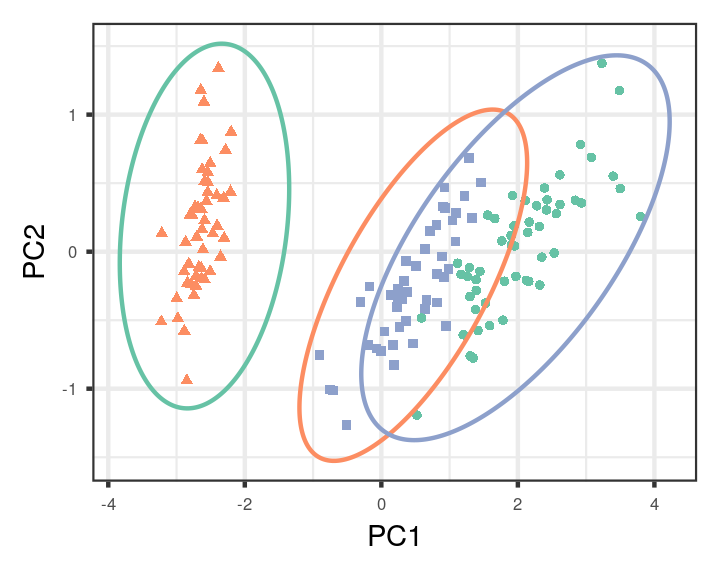
\includegraphics[width=0.588\linewidth,height=0.470\linewidth]{figure/iris_fit-1} 

}

\caption[The iris data in principal component space]{The iris data in principal component space. 
                      Colors denote inferred memberships and
                      ellipses are estimated covariances 
                      at $\alpha=6$.}\label{fig:iris_fit}
\end{figure}


\end{knitrout}


\begin{knitrout}
\definecolor{shadecolor}{rgb}{0.969, 0.969, 0.969}\color{fgcolor}\begin{figure}[!h]

{\centering 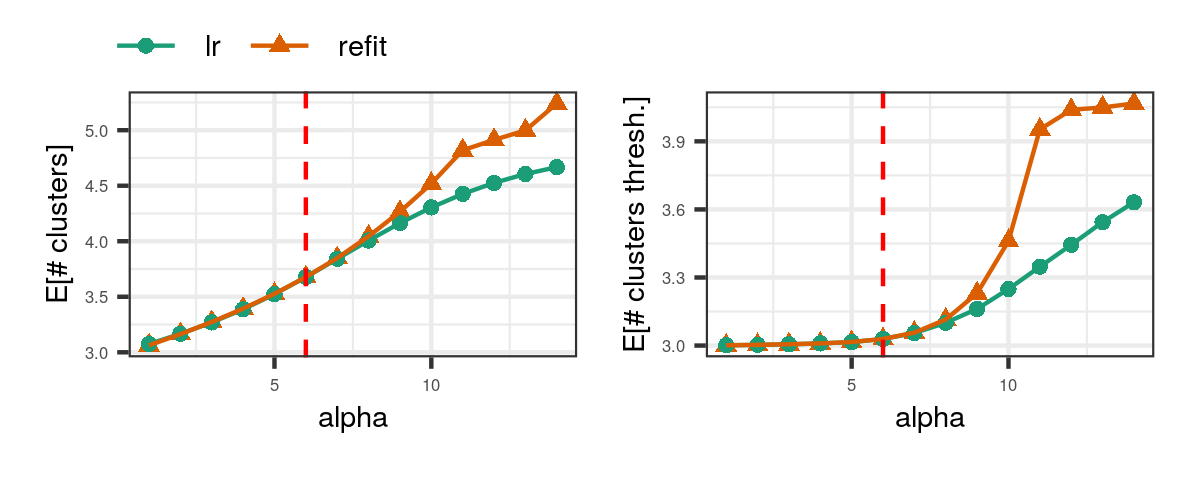
\includegraphics[width=0.980\linewidth,height=0.392\linewidth]{figure/iris_alpha_sens-1} 

}

\caption[The expected number of clusters in the iris data as $\alpha$ varies]{The expected number of clusters in the iris data as $\alpha$ varies. 
We compute the linear approximation at $\alpha=6$ and
extrapolate the expected number of clusters using the
linear approximation (green).
We compare against the expected number of clusters obtained by refitting the model at each $\alpha$ (orange). In the right plot, the threshold is set at $t = 1$. 
}\label{fig:iris_alpha_sens}
\end{figure}


\end{knitrout}



\begin{knitrout}
\definecolor{shadecolor}{rgb}{0.969, 0.969, 0.969}\color{fgcolor}\begin{figure}[!h]

{\centering 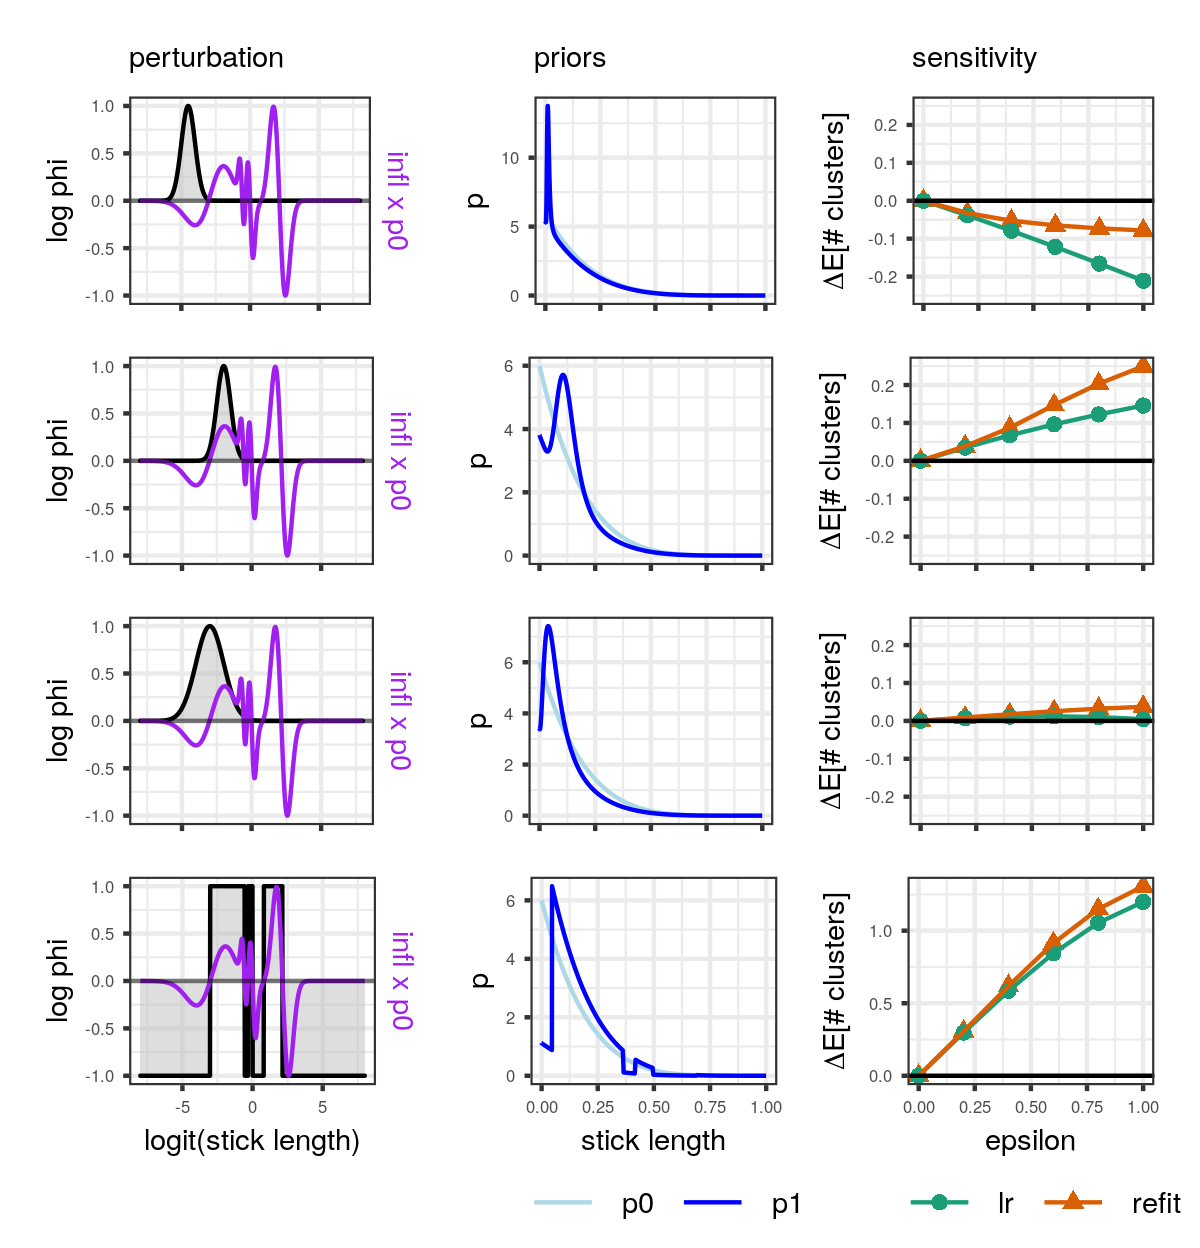
\includegraphics[width=0.980\linewidth,height=1.176\linewidth]{figure/iris_fsens-1} 

}

\caption[Demonstration of the influence function on 
        the expected number of clusters in the iris dataset]{Demonstration of the influence function on 
        the expected number of clusters in the iris dataset. 
        (Left) The influence function $I(x)$ 
        times the initial prior $p_0(x)$ at $\alpha = 6$. 
        We perturb $p_0$ with $\log \phi$ set to a step
        function with value one within the grey strips, and zero otherwise. 
        (Middle) The original prior density $p_0$ and the perturbed prior density $p_0\times \phi$. 
        (Right) The effect of the perturbation 
        on the change in expected number of clusters as $\epsilon \rightarrow 1$. }\label{fig:iris_fsens}
\end{figure}


\end{knitrout}


